\subsection{Performance measure of stateful operations on event attributes}
In this subsection, the performance of the stateful operations on event attributes is presented. This class of operation maintains the state for an event type and use the state to take a decision on a newly detected event of the time. The stateful operator that has been implemented is a moving maxima operation, which moves the maximum value for the event attribute each time a value greater than the last seen maximum value is encountered.
\subsubsection{Moving Maxima operator}
The Moving Maxima operator is denoted as:
\begin{equation}
D(e.t  \wedge (e.a_1  <=\quad \rightarrow maxvalue) ) \quad | \quad filter
\end{equation}\\
where \textit{D} is the detect operation; \newline
\textit{e.t} is the event type; \newline
\textit{e.a1} is the first event attribute; \newline
| denotes the redirect operation; \newline
and \textit{fliter} is the denotation for filtering of the event. \newline \newline
In this operation, all the events with attribute lower than the given \textit{maxvalue} are filtered. However, on the detection of an event with a value higher than the given \textit{maxvalue}, the event is forwarded, and the newly seen value becomes \textit{maxvalue}. 

In the first stage of evaluation, the same methodology used in section 5.4.8 is used. The rule installed in the switch to perform this operation is:
\begin{lstlisting}[language=json,firstnumber=1]
{
"dpid": 178974088016461,
"table_id": 0,
"priority": 11112,
"flags": 1,
"match":{
"dl_type":0x0800,
"nw_proto":17,
"nw_src":"10.1.1.2",
"nw_dst":"10.1.1.1",
"tp_dst":9877,
"e_type":"TEMP",
},
"actions":[{
"type":"SET_MOV_MAX",
"value": 20
},
]
}
http://localhost:8080/stats/flowentry/add \end{lstlisting}

Which in the perspective of event query languages can be represented as:

\begin{verbatim}
SET MAXVAL TEMPSTREAM CONDITION (20 < DEVICE_1.VALUE ? DEVICE_1.VALUE : 20)
DROP FROM TEMPSTREAM
WHERE DEVICE_1.VALUE < MAXVAL
\end{verbatim}

\subsubsection{Window Maxima operator}
\begin{equation}
D(e.t  \wedge (e.a_1  <=\quad \overrightarrow{win} \quad maxvalue)) \quad | \quad filter
\end{equation}\\
where \textit{D} is the detect operation; \newline
\textit{e.t} is the event type; \newline
\textit{e.a1} is the first event attribute; \newline
| denotes the redirect operation; \newline
and \textit{fliter} is the denotation for filtering of the event. \newline \newline
In this operation, the events with attribute lower than the given \textit{maxvalue} are filtered. However, on the detection of an event with a value higher than the given \textit{maxvalue}, the event is forwarded and the newly seen value becomes \textit{maxvalue}. The \textit{maxvalue} increases for a window of \textit{win} events after which it remains steady. if the window is 0, this is equivalent to less than or equal to operation defined in 5.11.

The rule installed in the switch to perform this operation is:
\begin{lstlisting}[language=json,firstnumber=1]
{
"dpid": 178974088016461,
"table_id": 0,
"priority": 11112,
"flags": 1,
"match":{
"dl_type":0x0800,
"nw_proto":17,
"nw_src":"10.1.1.2",
"nw_dst":"10.1.1.1",
"tp_dst":9877,
"e_type":"TEMP"
},
"actions":[
{
"type":"SET_WIN",
"val": 100
},
{
"type":"SET_MOV_MAX",
"val": 5
}
]
}

http://localhost:8080/stats/flowentry/add \end{lstlisting}

Which in the perspective of event query languages can be represented as:

\begin{verbatim}
SET MAXVAL TEMPSTREAM CONDITION (5 < DEVICE_1.VALUE ? DEVICE_1.VALUE : 5) WINDOW(100, TEMP) 
DROP FROM TEMPSTREAM
WHERE DEVICE_1.VALUE < MAXVAL
\end{verbatim}

\subsubsection{Performance of Stateful Operations}
Without accounting for accuracy, only events which will satisfy the rule each time are first forwarded. A stream of events with ever increasing attribute will always satisfy the rules described above. With such a set up the performance of the operations with bridged namespaces are measured and the plot in figure 5.13 captures the results observed. The point-to-point latency for stateful operations is marginally higher than the latency observed for compare operations because of the additional processing required to store and retrieve state for the event type.
\\
\begin{figure}[H]
	\centering
	\caption{Performance of stateful operations}
	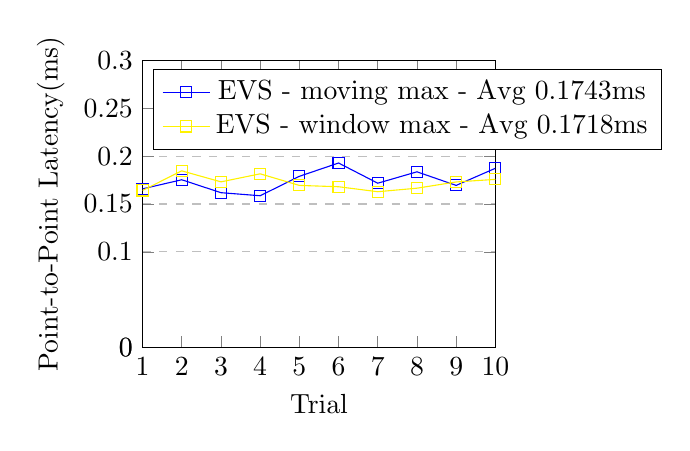
\begin{tikzpicture} [baseline=(current axis.outer east)]
	\begin{axis}[
	width=0.5\textwidth,
	xlabel={Trial},
	ylabel={Point-to-Point Latency(ms)},
	xmin=1, xmax=10,
	ymin=0.00, ymax=0.30,
	xtick={1,2,3,4,5,6,7,8,9,10},
	ytick={0.00,0,05,0.10,0.15,0.20,0.25,0.30},
	legend pos=north west,
	ymajorgrids=true,
	grid style=dashed,
	]
	\addplot[
	color=blue,
	mark=square,
	]
	coordinates {
		(1,0.1658)(2,0.1753)(3,0.1618)(4,0.1586)(5,0.1789)(6,0.1928)(7,0.1717)(8,0.1836)(9,0.1694)(10,0.1873)
		
	};
	\addlegendentry{EVS - moving max - Avg 0.1743ms}
	
	\addplot[
	color=yellow,
	mark=square,
	]
	coordinates {
		(1,0.1641)(2,0.1846)(3,0.1731)(4,0.1815)(5,0.1694)(6,0.168)(7,0.1628)(8,0.1665)(9,0.173)(10,0.1757)
		
		
	};
	\addlegendentry{EVS - window max - Avg 0.1718ms} 
	
	
	\end{axis}
	\end{tikzpicture}\hfill
	
\end{figure}


\subsection{Evaluating for accuracy - stateful operations}
In this subsection, the performance of stateful operations are measured with the settings for accuracy as decribed in section 5.4.9. As the results shown in section 5.4.9 show the accuracy of the operations depends on the caching mechanism used by Open vSwitch. To test the accuracy of stateful operation, the rule described by operation 5.12 is set up. The evntsrc is set up to send events with attribute described in below format:

\begin{lstlisting}[language=c]
/*
0,
0,1,
0,1,2,
0,1,2,3,
0,1,2,3,4,
...
...
0,1,2,3,.....               ...  , 96,
0,1,2,3,.....               ...  , 96,97,
0,1,2,3,.....               ...  , 96,97,98,
0,1,2,3,.....               ...  , 96,97,98,99
*/
\end{lstlisting}

while the evntsink compares the value of event attribute received to a counter which is incremented in a format described illustrated below:
\begin{lstlisting}[language=c]
/*
20,
20,21,
21,22,
23,23,
23,24,
..,
..,
95,96,
96,97,
97,98,
98,99,
99  
*/
\end{lstlisting}
if the received event attribute at each loop is lower than the loop counter, the received event is classified as a miss - i.e. an event which was supposed to be filtered by the EVS bridge, but wasn't. This form of evaluation ensures that the event rule installed in the EVS bridge is repeatedly forced to evaluate the event action, and also keep a deterministic baseline for comparison. For example in this setup, the total number of events transmitted is 5050; the total number of events to be passed through the moving max filter criteria is 159; At each iteration, if an event with attribute lower than the loop counter is seen, it is a miss. I.e., in the 20 loop, only event 20 is passed; in the 21st loop, events 20 and 21 are passed; in the 22nd loop, events 21 and 22 are passed; and so on. The evaluation is repeated for increasing values of event rate with two configurations:
\begin{itemize}
	\item Disabled Megaflows
	\item Max Idle Time 1 ms
\end{itemize}

\pgfplotstableread[row sep=\\,col sep=&]{
	Delay & Disabled & Max   \\
	7     & 92.45  & 82.38   \\
	8     & 96.85534591 & 80.50   \\
	9    & 95.59748428 & 92.45283019 \\
	10    & 96.85534591 & 98.11320755  \\
	11    & 94.96855346 & 98.74213836  \\
	12  &  94.96855346 & 99.37106918\\
}\delaydata




\begin{figure}[H]
	\noindent\hrulefill
	
	\noindent
	\caption{Accuracy of stateful operations}
	\begin{tikzpicture}
	\begin{axis}[
	ybar,
	xlabel={Delay in Rule hit (ms)},
	ylabel={Accuracy of compare operations(percentage)},
	symbolic x coords={7,8,9,10,11,12},
	nodes near coords,
	legend style={at={(0.5,1)},
		anchor=south,legend columns=-1},
	]
	\addplot[fill=green] table[x=Delay,y=Disabled]{\delaydata};
	\legend{Disabled Megaflow}
	\end{axis}
	\end{tikzpicture}
	\hfil
	\begin{tikzpicture}
	\begin{axis}[
	ybar,
	xlabel={Delay in Rule hit (ms)},
	ylabel={Accuracy of compare operations(percentage)},
	symbolic x coords={7,8,9,10,11,12},
	nodes near coords,
	legend style={at={(0.5,1)},
		anchor=south,legend columns=-1},
	]
	\addplot[fill=red ] table[x=Delay,y=Max]{\delaydata};
	\legend{Max Idle Time 1ms}
	\end{axis}
	\end{tikzpicture}
\end{figure}

As plotted in figures 5.14 and 5.15, the best accuracy and least latency is observed with a delay in rule hit of 12 ms and re-validator thread configure to collect every 1 ms. This observation is very similar to the accuracy evaluation of compare operations plotted in figure 5.10 and 5.11. The evaluation with a config time of 5 ms is avoided altogether because doing so made no difference during the evaluation of compare operations.

\begin{figure}[H] 
	\centering
	\caption{Performance of Stateful Operations}
	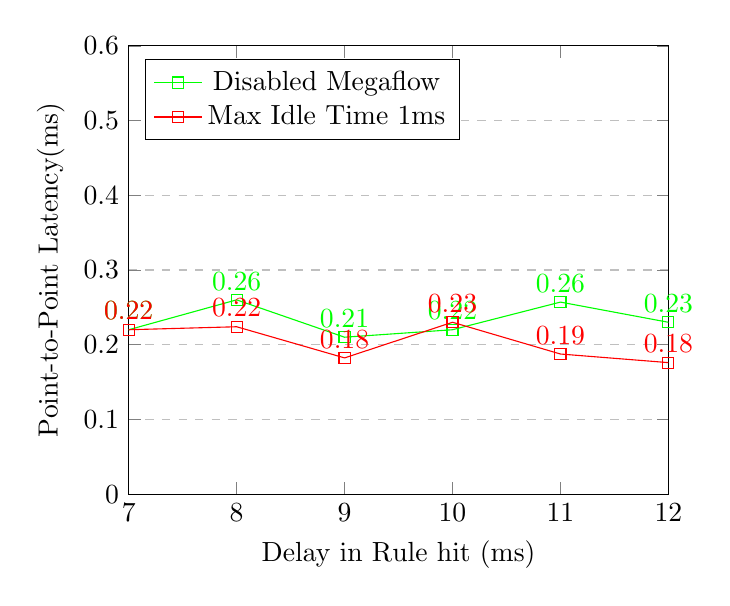
\begin{tikzpicture} 
	\begin{axis}[
	xlabel={Delay in Rule hit (ms)},
	ylabel={Point-to-Point Latency(ms)},
	xtick=data,
	xmin=7, xmax=12,
	ymin=0.00, ymax=0.6,
	xtick={7,8,9,10,11,12},
	ytick={0.00,0.10,0.20,0.30,0.40,0.50,0.60},
	nodes near coords,
	legend pos=north west,
	ymajorgrids=true,
	grid style=dashed,
	]
	\addplot[
	color=green,
	mark=square,
	]
	coordinates {
		(7,0.22)
		(8,0.26)
		(9,0.21)
		(10,0.22)
		(11,0.257)
		(12,0.23)
	};
	\addlegendentry{Disabled Megaflow} 
	
	\addplot[
	color=red,
	mark=square,
	]
	coordinates {
		(7,0.22)
		(8,0.224)
		(9,0.1823)
		(10,0.23)
		(11,0.1875)
		(12,0.176)
	};
	\addlegendentry{Max Idle Time 1ms} 
	\end{axis}
	\end{tikzpicture}
	
\end{figure} 

